\chapter{Spécifications géométriques et Chaînes de côte}
\thispagestyle{plain} % Supprimer le header & le footer sur cette page en laissant la numérotation
\newpage

%----------------------------------------------------------------------------------------
%	Spécifications géométriques
%----------------------------------------------------------------------------------------

\section{Spécifications géométriques}

\exercice{Dessin de définition}
Figure 1 - Dessin de définition du fourreau de lisse d'une barrière automatique
\begin{center}
    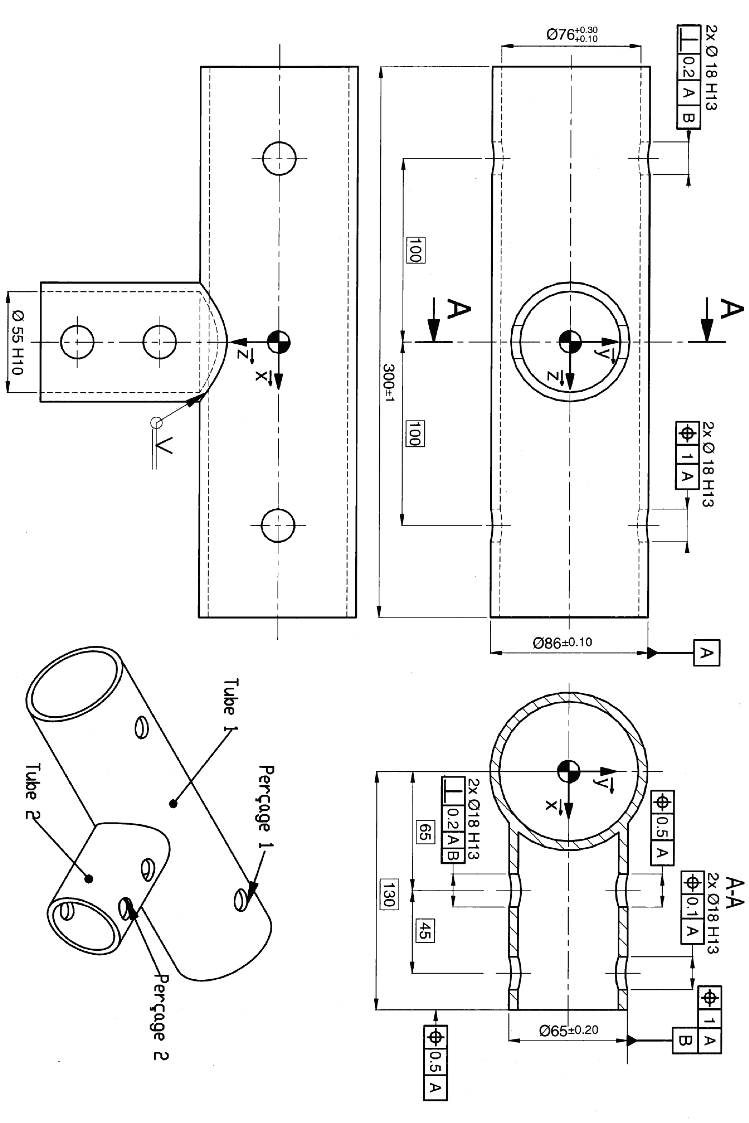
\includegraphics[scale=0.5]{png/tube.png}
\end{center}
\newpage

\subsubsection{Travail demandé}
Compléter le tableau ci-dessous pour les spécifications géométriques suivantes : 
\begin{center}
    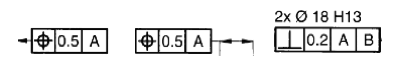
\includegraphics[scale=0.5]{png/tube_data.png}
\end{center}
\begin{center}
    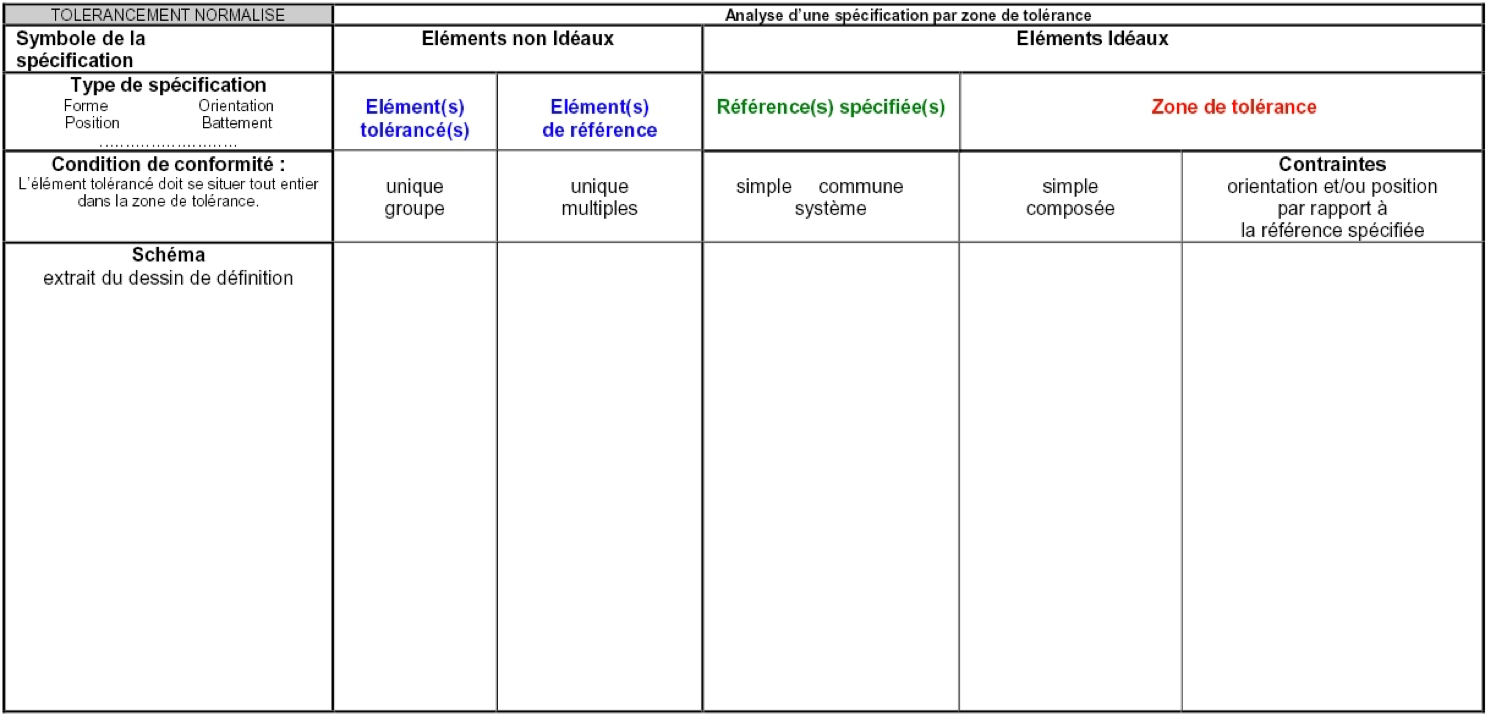
\includegraphics[scale=0.65]{png/doc_rep.png}
\end{center}

\newpage

%--------------------------------------------

\exercice{Vue partielle d'un marbre}

Figure 1 - Vue partielle d'un marbre
\begin{center}
    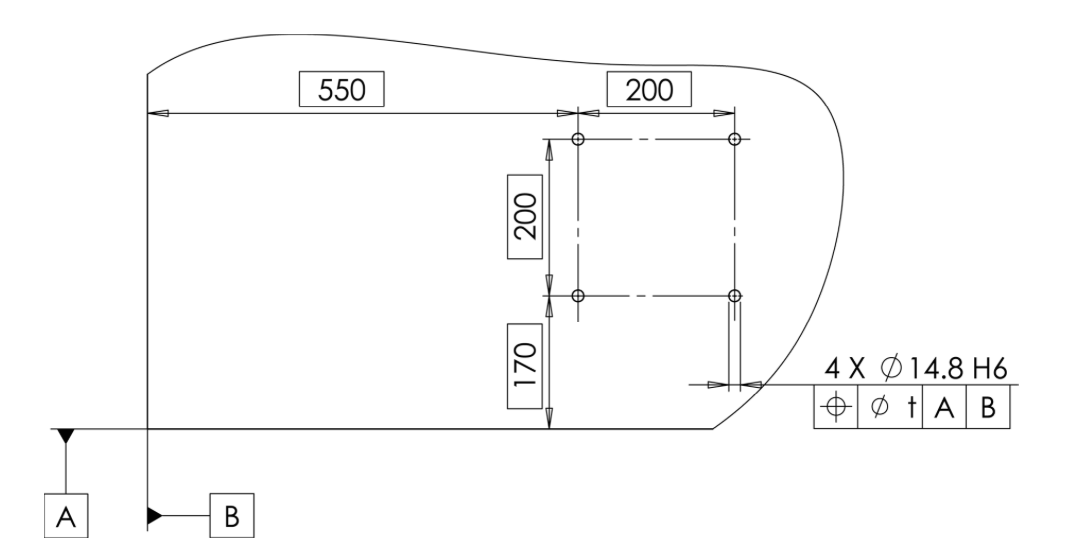
\includegraphics[scale=0.5]{png/marbre.png}
\end{center}

\subsubsection{Travail demandé}
Compléter le tableau suivant pour la spécification de la Figure 1 :
\begin{center}
    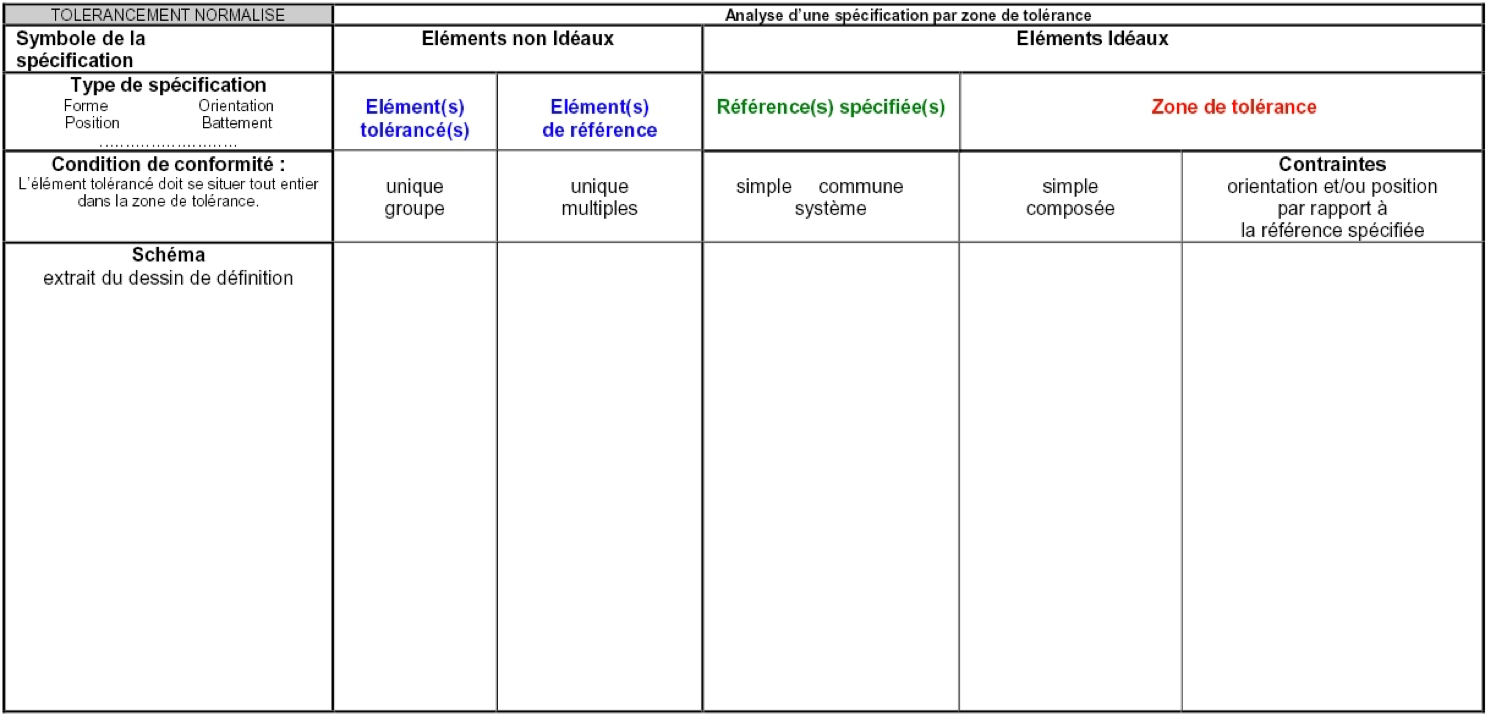
\includegraphics[scale=0.65]{png/doc_rep.png}
\end{center}

\newpage

%----------------------------------------------------------------------------------------
%	Chaînes de côtes
%----------------------------------------------------------------------------------------

\section{Chaînes de côte}

\exercice{Assemblage avec clavette}
L'arbre de la Figure $1$ présente une certaine fréquence de rotation $N$. A
l'aide d'un assemblage par clavette, la roue dentée, fixée sur l'arbre, a la même fréquence de rotation.

\begin{center}
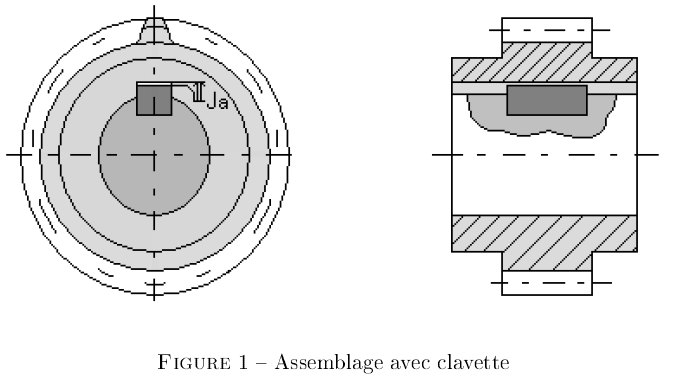
\includegraphics[scale=0.5]{png/clavette.png}
\end{center}

\subsubsection{Travail demandé}
\begin{enumerate}
\item Tracer la chaîne de côte. (chaque pièce apparaisse une seule fois)
\item Donner les expressions pour le jeu $J_a$, du jeu maximal et minimal.
\end{enumerate}

\correction{ 
\begin{center}
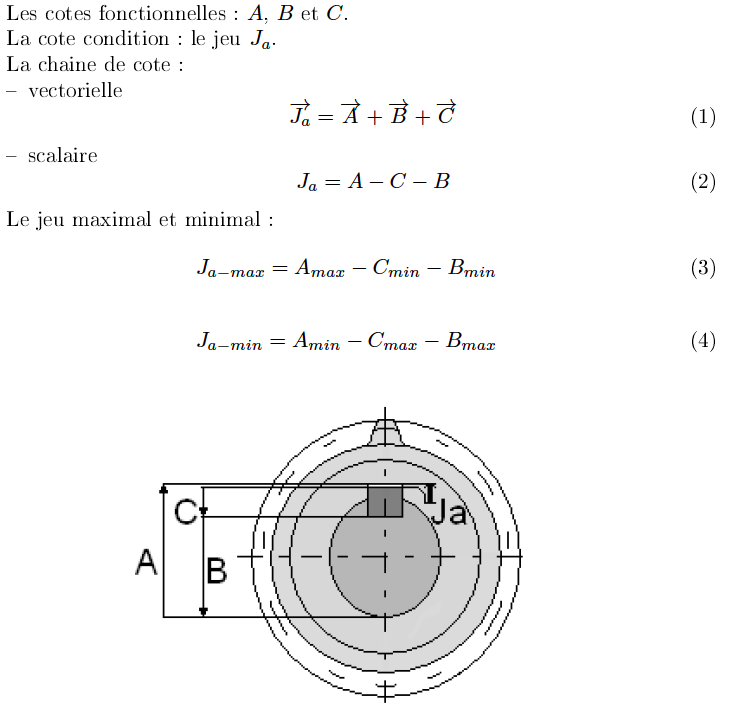
\includegraphics[scale=0.55]{png/sol1.png}
\end{center}
}
\newpage

%--------------------------------------------

\exercice{Arbre - Roues dentées - Roulements}
Le mécanisme de la figure $2$ est formé par un arbre, $2$ roues dentées, une
clavette, $2$ roulements et un joint en caoutchouc.

\begin{center}
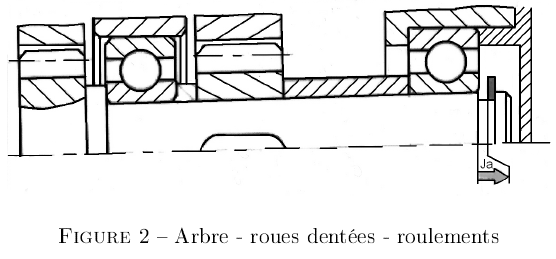
\includegraphics[scale=0.5]{png/arbre.png}
\end{center}

\subsubsection{Travail demandé}
\begin{enumerate}
\item Tracer la chaîne de côte.
\item Donner les expressions pour le jeu $J_a$, du jeu maximal et minimal.
\end{enumerate}

\correction{ 
\begin{center}
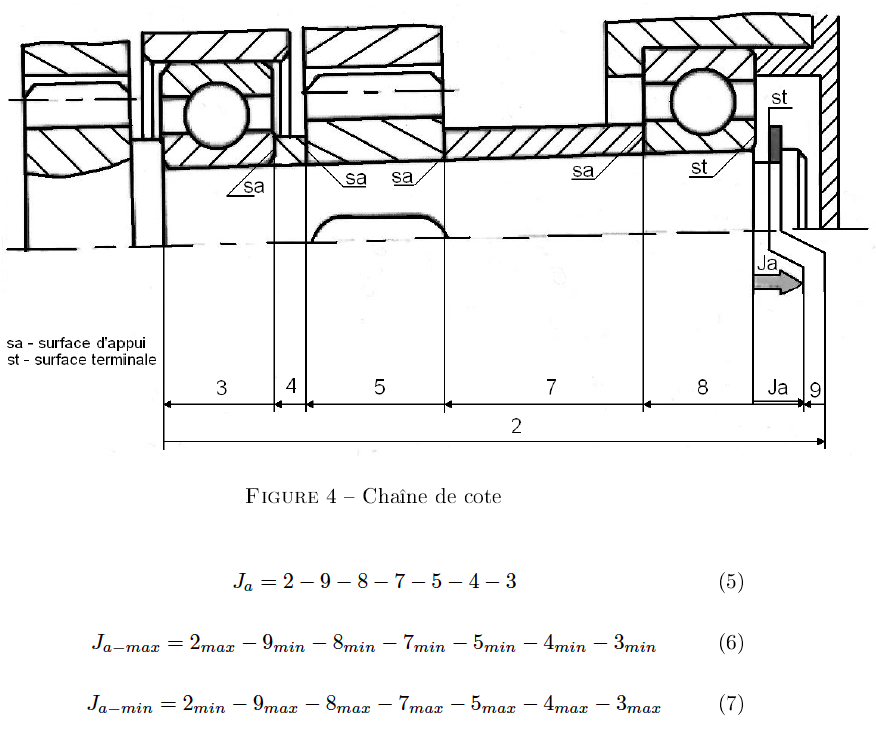
\includegraphics[scale=0.5]{png/sol2.png}
\end{center}
}
\newpage

%--------------------------------------------

\exercice{Blocs}
\begin{center}
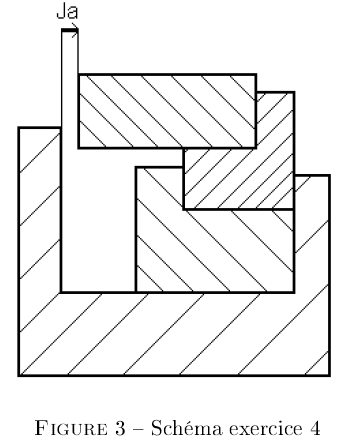
\includegraphics[scale=0.5]{png/box.png}
\end{center}

\subsubsection{Travail demandé}
\begin{enumerate}
\item Tracer la chaîne de côte du jeu $J_a$ sur la figure $4$.
\item Donner les expressions pour le jeu $J_a$, du jeu maximal et minimal.
\end{enumerate}

\correction{ 
\begin{center}
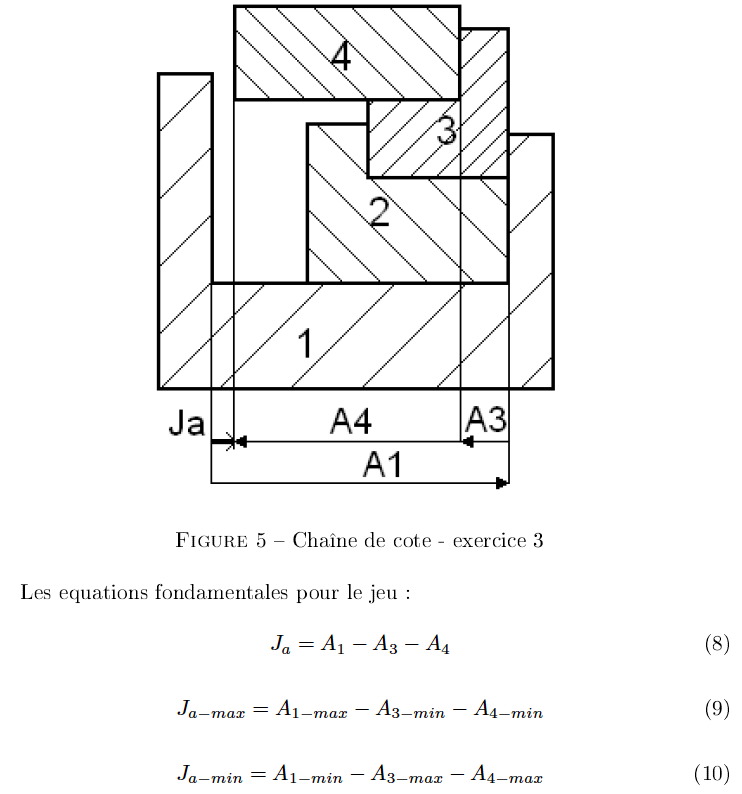
\includegraphics[scale=0.4]{png/sol3.png}
\end{center}
}
\newpage

%----------------------------------------------------------------------------------------
%	Problèmes
%----------------------------------------------------------------------------------------

\section{Problèmes}

\probleme{Micromoteur deux temps}
Le mécanisme décrit ci-dessous constitue le support des exercices d'application à l'écriture des spécifications.\\
Il s'agit d'un micro moteur $2$ temps d'une cylindrée de $5 cm^3$ utilisé en micro modélisme. Cet ensemble est présenté dans le dessin en coupe figuré ci-dessous.

\begin{center}
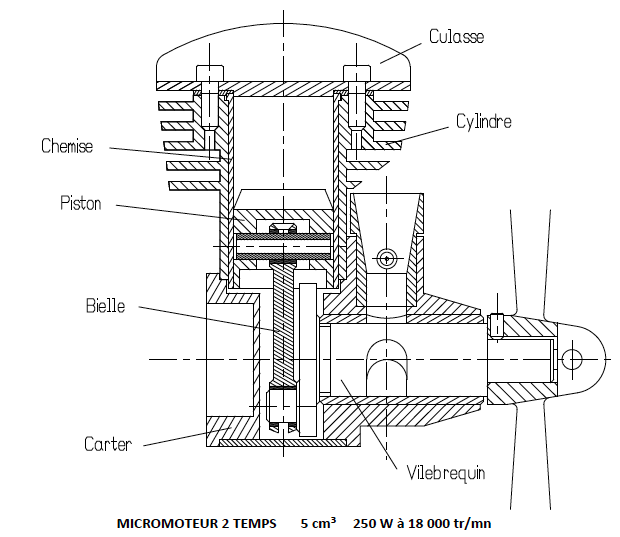
\includegraphics[scale=0.65]{png/moteur2temps.png}
\end{center}

Les conditions fonctionnelles attachées à ce mécanisme sont nombreuses : étanchéité, pression de contact entre surfaces, comportement de la chaîne cinématique, faisabilité de l'assemblage, etc. \dots\\
De cet ensemble de conditions, se déduit toute une série de contraintes dimensionnelles et géométriques attachées aux éléments non idéaux extraits du "Skin Modèle" des diverses pièces constitutives de ce mécanisme.\\
Ce sont ces contraintes qui font l'objet des spécifications à formuler dans les divers exercices qui suivent. L'expression devra se faire dans le respect le plus strict des normes en vigueur.

\newpage
\subsubsection{Partie 1 -- Vilbrequin}
Une partie des exigences concourant au bon fonctionnement du mécanisme (guidage en rotation, pression de contact, respect de la course et du taux de compression) conduit à imposer :

\begin{itemize}
\item une spécification par dimension portant sur le diamètre du tourillon de vilebrequin
\item une spécification par zone de tolérance portant sur la forme de ce tourillon
\item une spécification par zone de tolérance portant sur la position du maneton par rapport au tourillon
\end{itemize}

\begin{enumerate}
\item Porter sur la figure ci-dessous les spécifications imposées par l'extrait du cahier des charges
présenté en préambule.\\
La formulation de ces spécifications devra respecter les règles du Tolérancement Normalisé.

\begin{center}
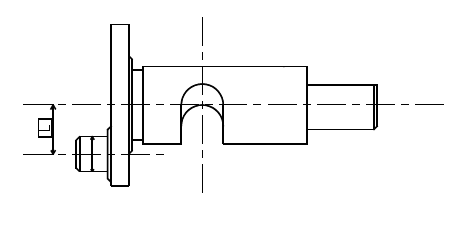
\includegraphics[scale=0.8]{png/vilbrequin.png}
\end{center}

\item Pour chacune des spécifications écrites, décrire son interprétation suivant la norme en vous appuyant sur le tableau suivant.

\begin{center}
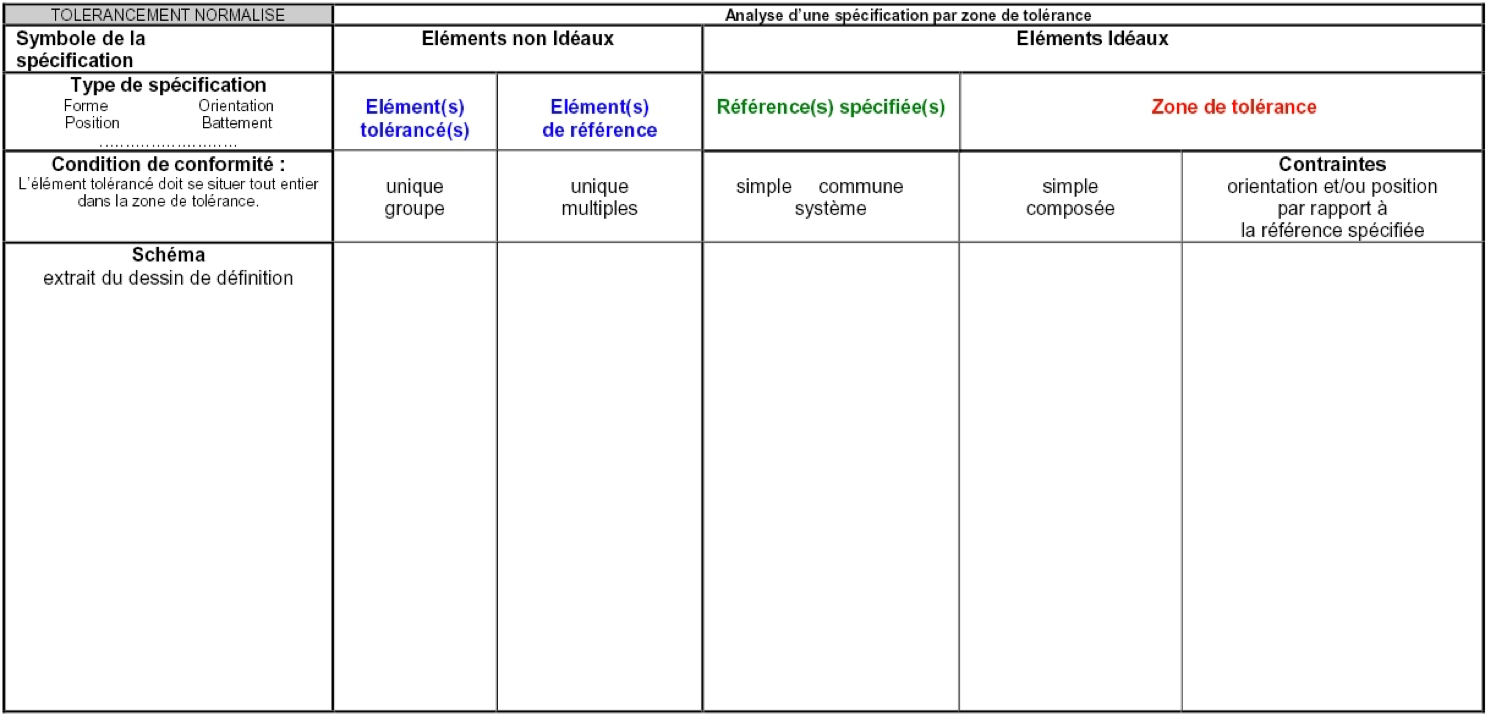
\includegraphics[scale=0.55]{png/doc_rep.png}
\end{center}

\end{enumerate}

\newpage
\subsubsection{Partie 2 -- Le carter}
Parmi les nombreuses exigences conduisant à un coulissement satisfaisant du piston dans le cylindre chemisé, le sujet propose de retenir celles qui s'attachent à maîtriser la qualité de la liaison entre cylindre et carter. Ainsi, parmi les spécifications attachées au carter :
\begin{itemize}
\item une première spécification définira le tolérancement de forme de la face d'appui du cylindre sur le carter,
\item une seconde spécification définira le tolérancement d'orientation de cette face d'appui par rapport à l'alésage recevant le coussinet guidant le tourillon du vilebrequin,
\item une troisième spécification définira le tolérancement de position de cette face par rapport à ce même alésage.
\item \underline{Nota :} Le carter sera considéré monobloc : Les pièces constitutives sont réunies, positionnées et usinées conjointement.
\end{itemize}

\begin{enumerate}
\item Porter sur la figure ci-dessous les spécifications imposées par l'extrait du cahier des charges
présenté en préambule.\\
La formulation de ces spécifications devra respecter les règles du Tolérancement Normalisé.

\begin{center}
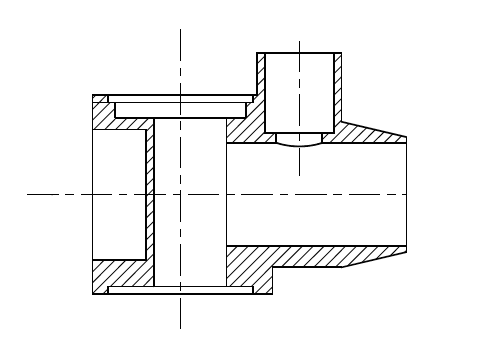
\includegraphics[scale=0.6]{png/carter2.png}
\end{center}

\item Pour chacune des spécifications écrites, décrire son interprétation suivant la norme en vous appuyant sur le tableau suivant.

\begin{center}
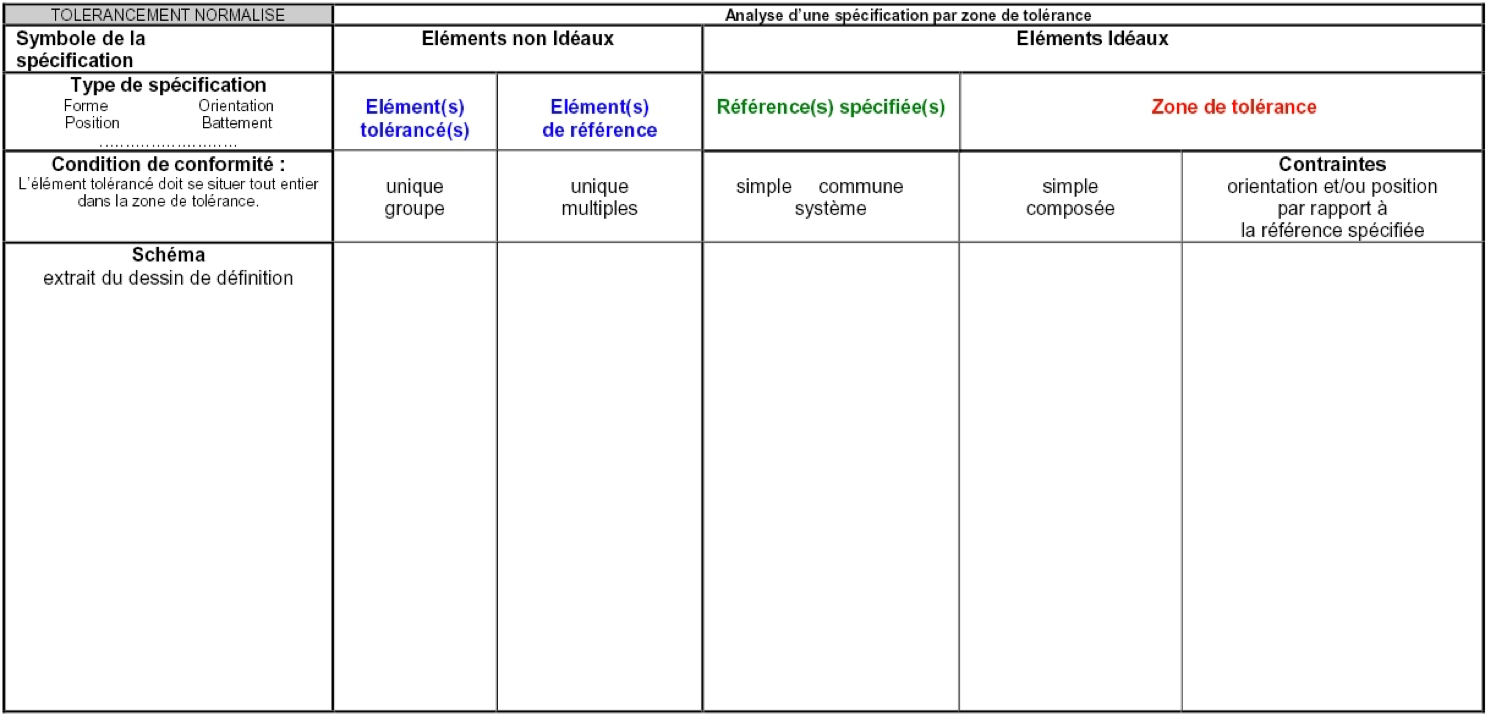
\includegraphics[scale=0.55]{png/doc_rep.png}
\end{center}
\end{enumerate}

\newpage
\subsubsection{Partie 3 -- Le cylindre}
En gardant le même objectif d'un coulissement satisfaisant du piston dans le cylindre chemisé, le sujet propose de définir une première spécification portant sur l'orientation de l'alésage recevant la chemise par rapport à la face d'appui du cylindre sur le carter.\\
De plus, la culasse est centrée dans la chemise puis fixée sur le cylindre par quatre vis. En conséquence, une seconde spécification s'attache à exprimer la localisation des quatre trous taraudés permettant l'implantation de ces vis dans le cylindre.

\begin{enumerate}
\item Porter sur la figure ci-dessous les spécifications imposées par l'extrait du cahier des charges
présenté en préambule.\\
La formulation de ces spécifications devra respecter les règles du Tolérancement Normalisé.

\begin{center}
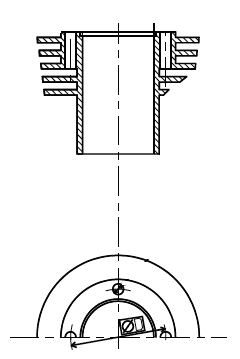
\includegraphics[scale=0.7]{png/cylindre.png}
\end{center}

\item Pour chacune des spécifications écrites, décrire son interprétation suivant la norme en vous appuyant sur le tableau suivant.

\begin{center}
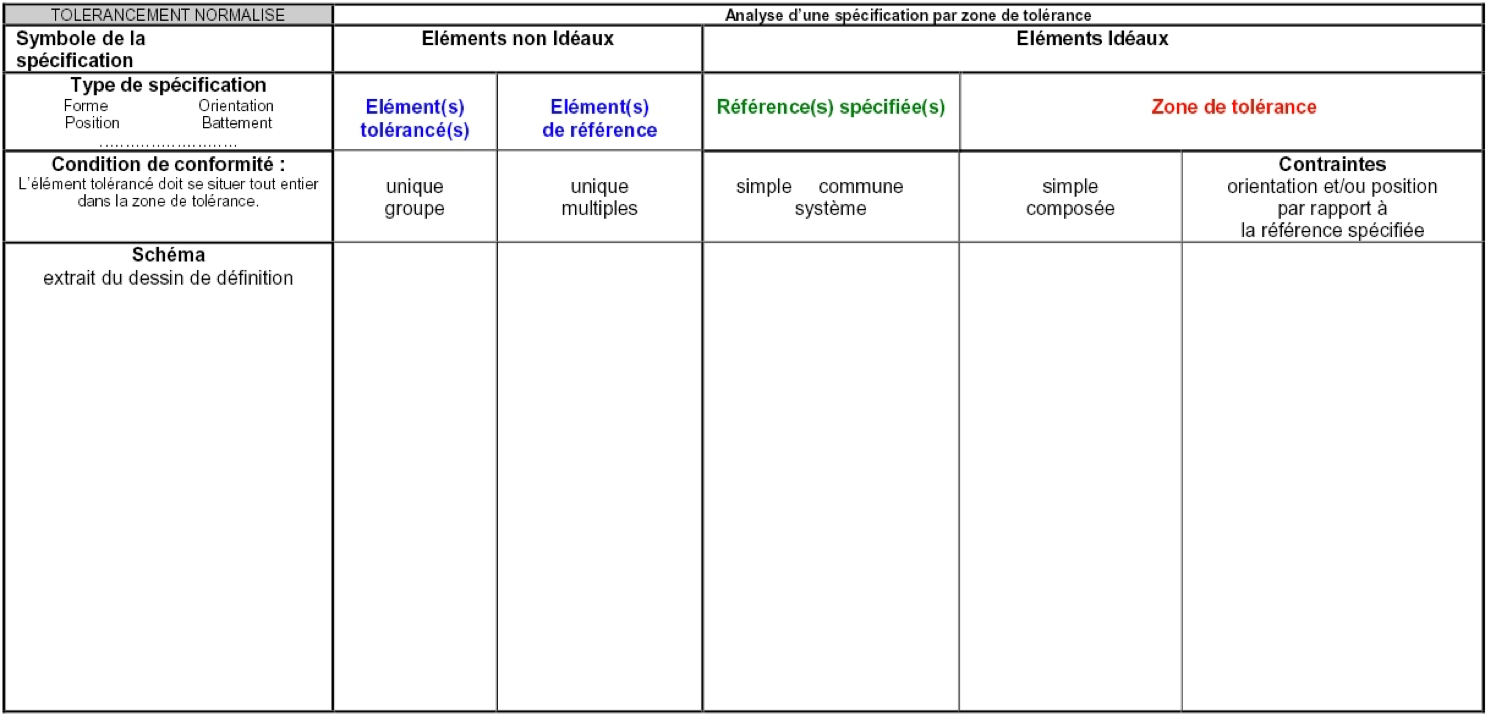
\includegraphics[scale=0.55]{png/doc_rep.png}
\end{center}
\end{enumerate}

\newpage
\subsubsection{Partie 4 -- La bielle}
Le caractère hyperstatique de la chaîne cinématique Cylindre-Piston-Bielle-Vilebrequin-Carter est flagrant.\\
Le bon fonctionnement de celle-ci ne peut être garanti sans une géométrie soignée de l'ensemble en association avec des jeux judicieusement quantifiés.\\
Ainsi, dans le dessin de définition de la bielle, une spécification par zone de tolérance doit exprimer l'orientation relative des alésages de tête et de pied de bielle.\\
D'autre part, le respect du taux de compression impose une spécification portant sur l'entraxe de ceux-ci.\\
\underline{Nota :} On pourra considérer que l'alésage de tête de bielle joue un rôle prioritaire dans la situation de la bielle dans le mécanisme.

\begin{enumerate}
\item Porter sur la figure ci-dessous les spécifications imposées par l'extrait du cahier des charges
présenté en préambule.\\
La formulation de ces spécifications devra respecter les règles du Tolérancement Normalisé.

\begin{center}
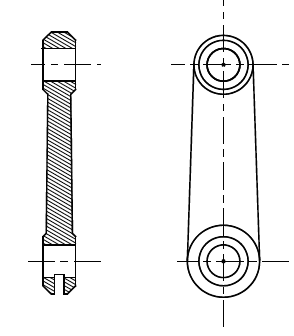
\includegraphics[scale=0.7]{png/bielle2.png}
\end{center}

\item Pour chacune des spécifications écrites, décrire son interprétation suivant la norme en vous appuyant sur le tableau suivant.

\begin{center}
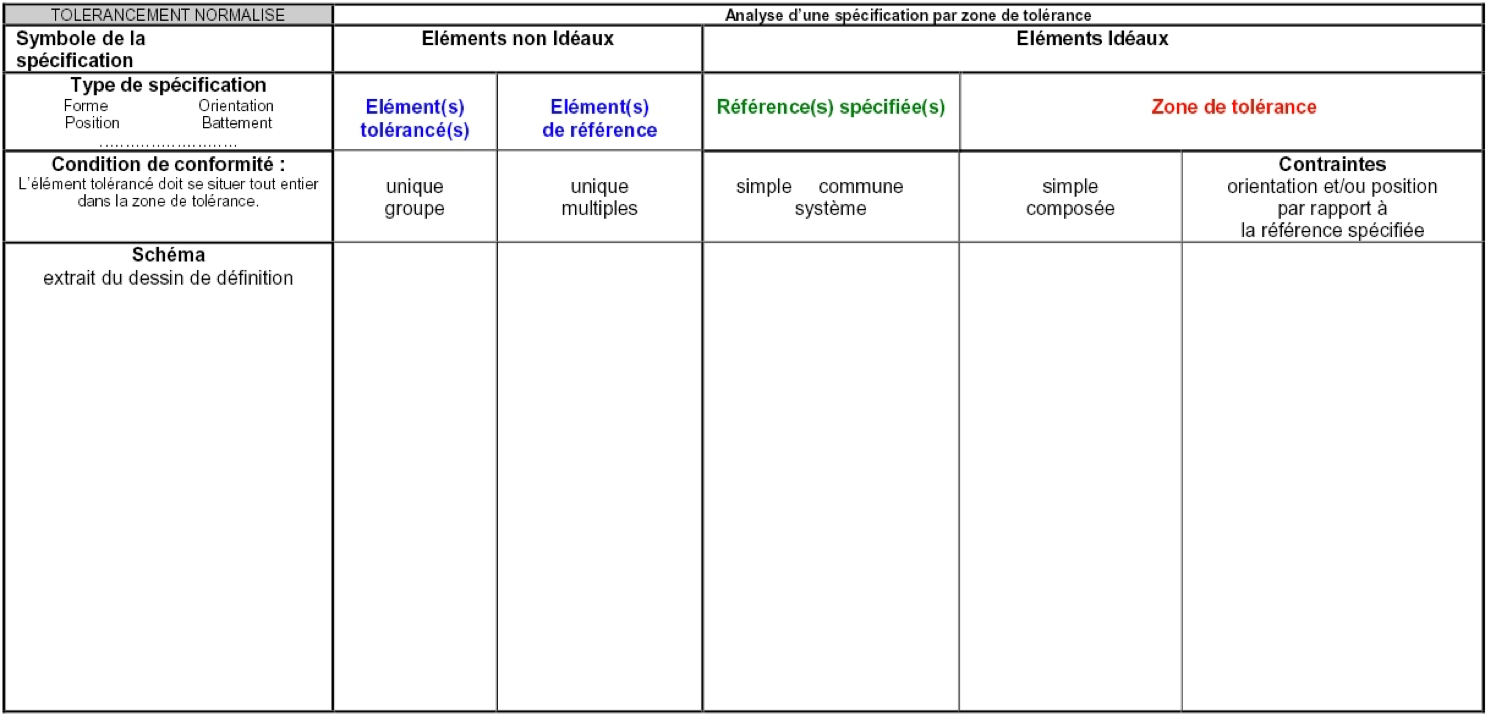
\includegraphics[scale=0.55]{png/doc_rep.png}
\end{center}
\end{enumerate}


\newpage
\subsubsection{Partie 5 -- Le piston}
Les contraintes liées à la liaison pivot glissant établie entre piston et chemise sont nombreuses :

\begin{itemize}
\item qualité du guidage
\item étanchéité dynamique
\item résolution de l'hyperstaticité
\end{itemize}

Il s'agit de spécifications par dimension et de spécifications par zone de tolérance (forme, orientation).

\begin{enumerate}
\item Porter sur la figure ci-dessous les spécifications imposées par l'extrait du cahier des charges
présenté en préambule.\\
La formulation de ces spécifications devra respecter les règles du Tolérancement Normalisé.

\begin{center}
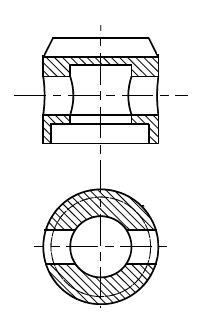
\includegraphics[scale=0.8]{png/piston.png}
\end{center}

\item Pour chacune des spécifications écrites, décrire son interprétation suivant la norme en vous appuyant sur le tableau suivant.

\begin{center}
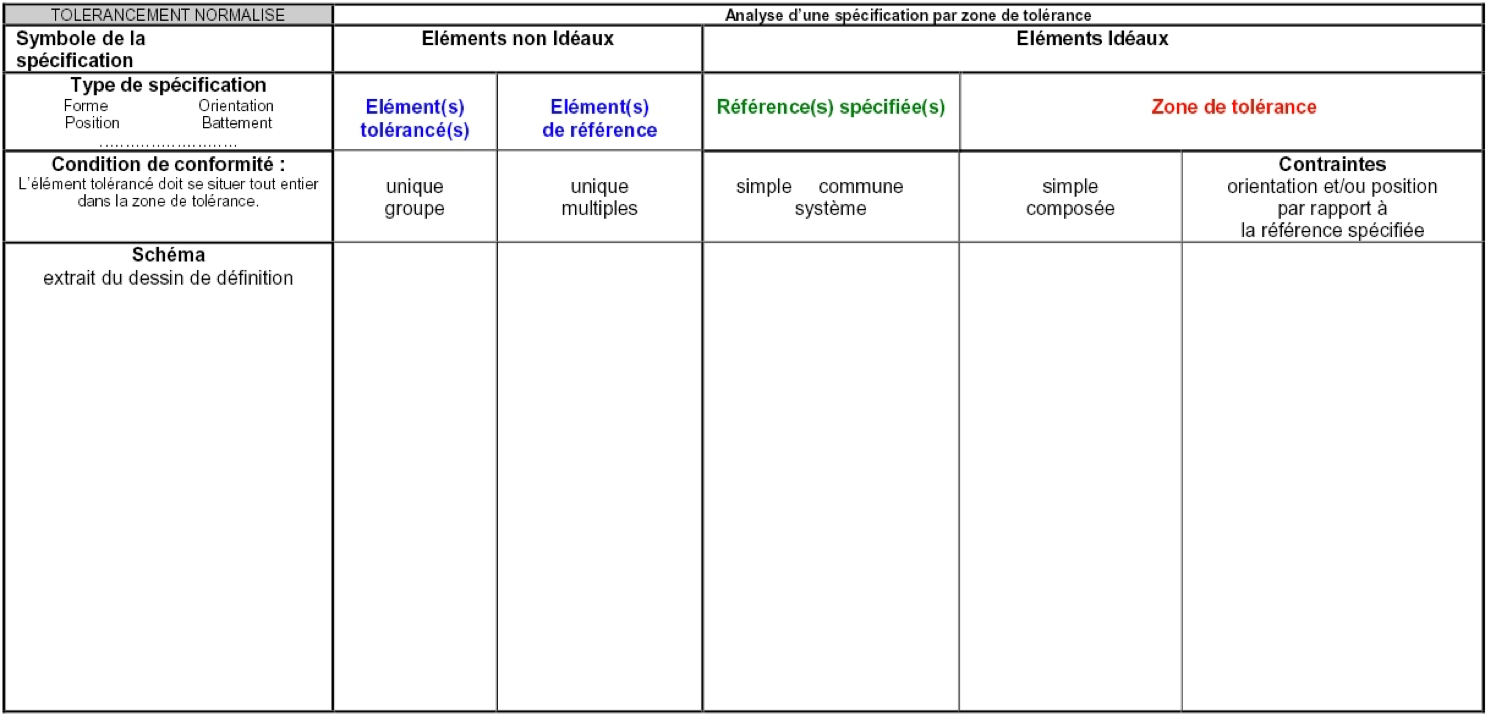
\includegraphics[scale=0.55]{png/doc_rep.png}
\end{center}
\end{enumerate}

%\correction{
%\textbf{Partie 1}
%\begin{enumerate}
%
%\item Figure :
%\begin{center}
%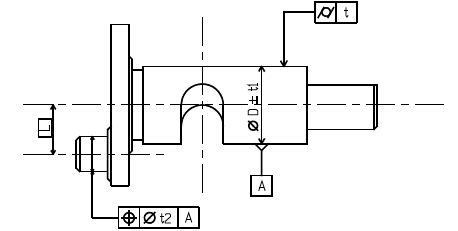
\includegraphics[scale=0.7]{png/vilbrequin-cor.png}
%\end{center}
%
%\item Spécifications :
%\begin{itemize}
%\item Spécification par dimension portant sur le diamètre du tourillon : Cette spécification impose à toute distance locale du type "diamètre" définie entre deux points extraits de la surface nominalement cylindrique (élément non idéal) d'avoir une valeur comprise entre $D - t_1$ et $D + t_1$.
%\item Spécification par zone de tolérance portant sur la forme du tourillon : Cette spécification de CYLINDRICITE attachée à l'élément tolérancé surface nominalement cylindrique impose à cet élément de se situer dans un espace de type volume limité par deux cylindres coaxiaux de différence de rayon $t$.
%\item Spécification par zone de tolérance portant sur la position du maneton : Cette spécification de POSITION attachée à l'élément tolérancé surface nominalement cylindrique impose à l'axe de cet élément de se situer dans un espace de type volume limité par un cylindre de diamètre $t_2$ d'axe contraint parallèle à DROITE $A$ et à distance $L$ de DROITE $A$ , axe du cylindre associé à l'élément de référence surface nominalement cylindrique repérée $A$.
%\end{itemize}
%
%%\begin{center}
%%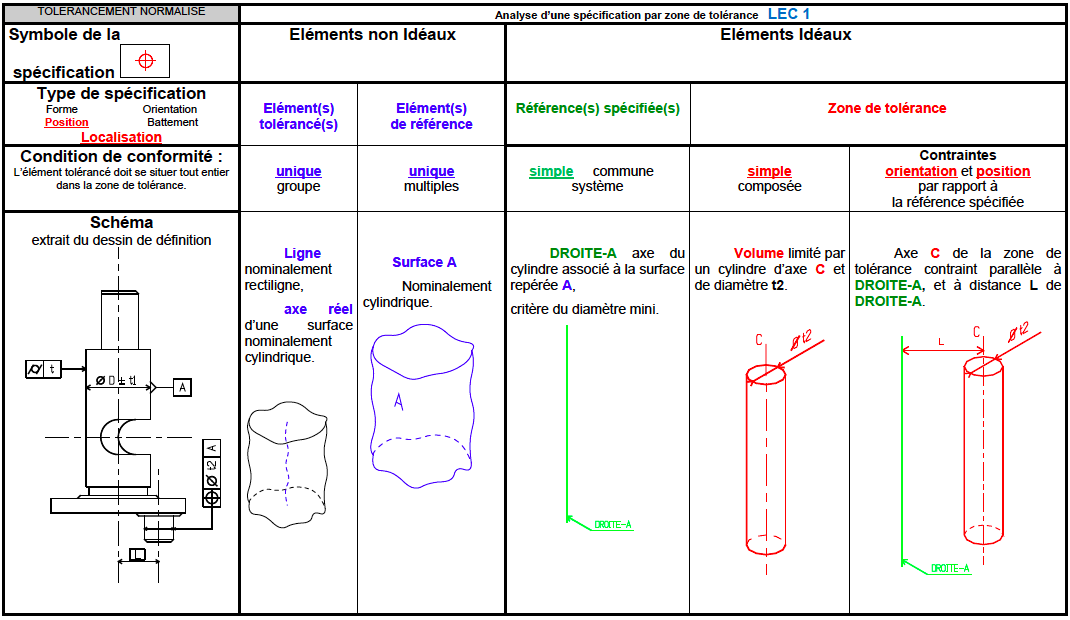
\includegraphics[scale=0.4]{png/cor-spe1.png}\\
%%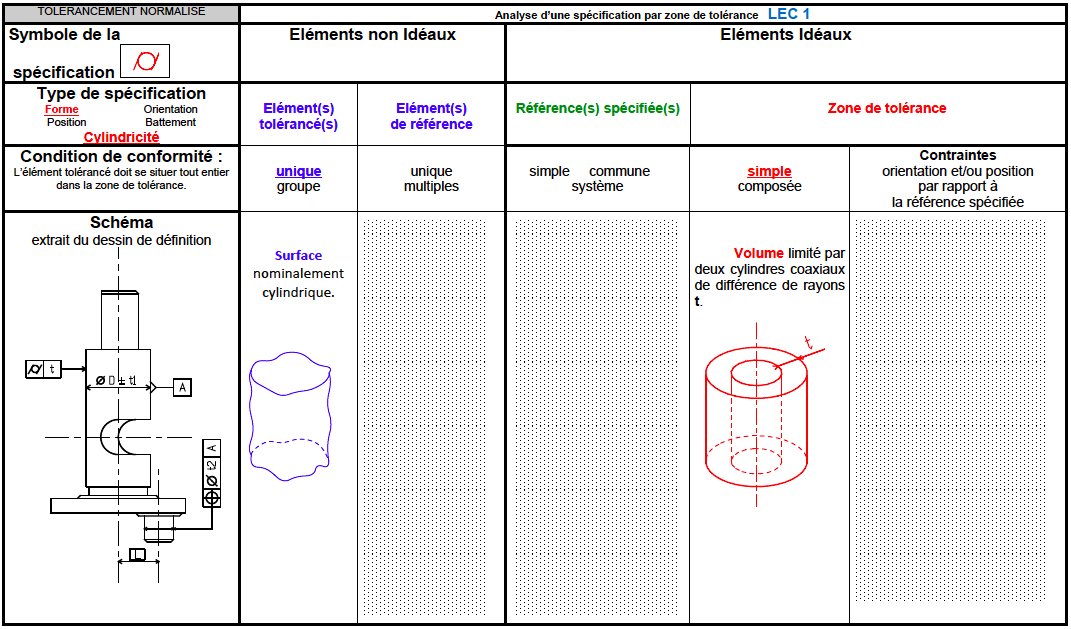
\includegraphics[scale=0.4]{png/cor-spe2.png}
%%\end{center}
%
%\end{enumerate}
%
%\textbf{Partie 2} 
%\begin{enumerate}
%\item Figure :
%\begin{center}
%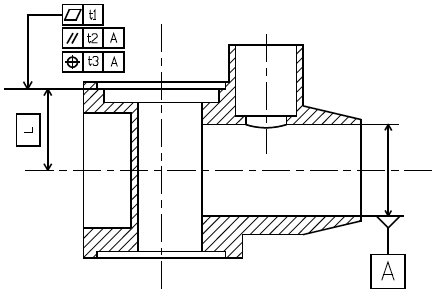
\includegraphics[scale=0.6]{png/carter-cor.png}
%\end{center}
%\item ?
%\end{enumerate}
%
%
%\textbf{Partie 3}
%\begin{enumerate}
%\item Figure :
%\begin{center}
%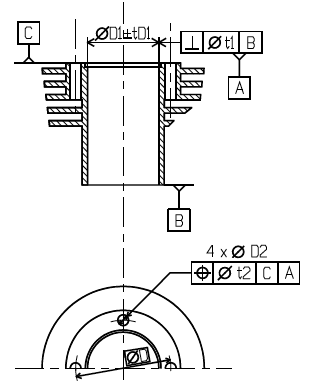
\includegraphics[scale=0.7]{png/cylindre-cor.png}
%\end{center}
%\item ?
%\end{enumerate}
%
%\textbf{Partie 4}
%\begin{enumerate}
%\item Figure :
%\begin{center}
%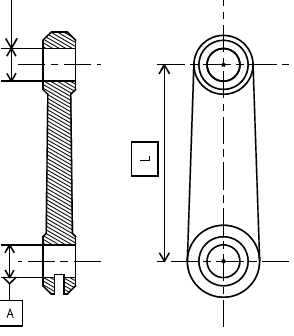
\includegraphics[scale=0.7]{png/bielle-cor.png}
%\end{center}
%\item ?
%\end{enumerate}
%
%\textbf{Partie 5}
%\begin{enumerate}
%\item Figure :
%\begin{center}
%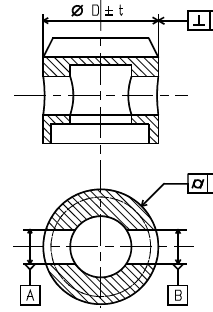
\includegraphics[scale=0.7]{png/piston-cor.png}
%\end{center}
%\item ?
%\end{enumerate}
%}
